
\subsection{Introduction aux ondes gravitationnelles}
\label{sec:introgw}

% origin
Détectées pour la première fois en 2015, les ondes gravitationnelles étaient prédites par la theorie de la relativité générale depuis 1916.
Une manière ``simple'' de les faire apparaître dans les équations de la relativité générale est en introduisant une perturbation dans la métrique d'un espace-temps plat.
Des calculs et changements de coordonnées, qui ne seront pas détaillé dans ce document, permettent d'arriver à une équation d'onde dont la métrique de l'espace-temps est solution.
Les ondes gravitationnelles sont à la relativité générale ce que les ondes électromagnétiques sont à l'électromagnétisme.
Tout comme la lumière, elles se propagent à la vitesse de la lumière dans le vide.
Cependant leur natures diffèrent grandement.
Dans le cas des ondes gravitationnelles c'est la courbure de l'espace-temps elle-même qui suit cette équation d'onde.
Cela implique que les ondes gravitationnelles se propagent à travers la matière sans altération.
Elles peuvent toutefois être modifiées par de forts champs gravitationnels créés par des objets très massifs.

% effects
Bien que se propageant au travers de l'espace-temps, elles n'affectent au premier ordre que les composantes spatiales de la métrique.
Elles n'ont d'effets que dans le plan transverse à leur direction de propagation.
Ainsi, deux particules ponctuelles séparées dans l'espace uniquement le long de la direction de propagation de l'onde gravitationnelle ne subiront aucun effet.
En revanche des particules séparées le long de directions transverses verront leur distance propre osciller proportionnellement à leur distance et l'amplitude de l'onde et selon la fréquence de cette dernière.

% transition to sources
De la même manière que des charges électriques en accélération émettent de la lumière en électromagnétisme, des masses en accélération produisent des ondes gravitationnelles.
L'amplitude des ondes est extrêmement faible et croît avec la masse de l'objet accéléré.
Pour pouvoir être détecté sur Terre, nous nous attendons donc à ce que l'objet en question soit très massif.


%%%%%%%%%%
\subsection{Aperçu des sources astrophysiques}
\label{sec:sources}

Cette section présente les principales sources d'ondes gravitationnelles qui sont recherchées par la collaboration LIGO-Virgo-KAGRA (LVK).

\subsubsection*{Les coalescences de paire d'objets compacts}

La première détection d'ondes gravitationnelles a été identifiée comme provenant d'une coalescence de binaire compact (CBC) qui consiste en la coalescence de deux objets compacts.
Dans le cas de cette première détection, appellée GW150914 en référence à la date de l'observation, la forme des signaux observés a permis de conclure qu'il s'agissait de deux trous noirs.
On parle alors de binaire de trous noirs (Binary Black Hole, BBH).
D'autres types de binaires étaient attendues comme les binaires d'étoiles à neutron (Binary Neutron Star, BNS) ou encore les binaires trou noir-étoile à neutron (Neutron Star-Black Hole, NSBH).
Il fallut attendre 2017 et 2020 respectivement pour la première observation d'une BNS et d'une NSBH.

Le processus de coalescence d'une CBC consiste en trois étapes:
\begin{itemize}

\item La phase spiralante ou ``Inspiral'': les deux objets sont en rotation l'un autour de l'autre à grande vitesse.
  Ils se rapprochent graduellement et leurs vitesses augmentent, atteignant des valeurs du même ordre de grandeur que la vitesse de la lumière dans le vide.
  Des ondes gravitationnelles sont émises tout au long de ce processus.
  La fréquence et l'amplitude des ondes augmentent à mesure que les objects se rapprochent et accélèrent.
  
\item La phase de fusion ou `` Merger'': les deux objets se sont tellement rapprochés qu'ils ont atteint leur dernière orbite circulaire stable (Innermost Stable Circular, Orbit, ISCO).
  Ils ``plongent'' l'un vers l'autre et fusionnent rapidement.
  C'est à ce moment que le signal gravitationnel atteint son amplitude et sa fréquence maximale.
  Le corps résultant de la fusion dépend du système initial.
  Dans le cas d'une BBH il s'agira d'un trou noir plus massif.
  Pour une NSBH le trou noir va disloquer et absorber l'étoile à neutron, résultant à nouveau en un trou noir.
  Plusieurs scénarios sont possible lorsque l'on considère une BNS.
  L'objet final peut être un trou noir ou une étoile à neutron.
  S'il s'agit d'une étoile à neutron elle pourrait par la suite s'effondrer et former un trou noir.
  Cet effondrement peut arriver en quelques secondes ou bien sur une durée plus longue.
  Ces scénarios dépendent des propriétés des deux étoiles initiales et de l'objet résultant de la fusion.
  
\item La phase de désexcitation ou ``Ringdown'': Cette étape n'est pertinente que si l'objet résultant est un trou noir massif.
  Suite à la fusion, le trou noir est dans un état excité et peut être très asymétrique.
  Il va radier de l'énergie par émission gravitationnelle jusqu'à atteindre un état d'équilibre.
\end{itemize}

La figure \ref{fig:inspiral} montre une représentation du processus complet.
%
\begin{figure}
  \centering
  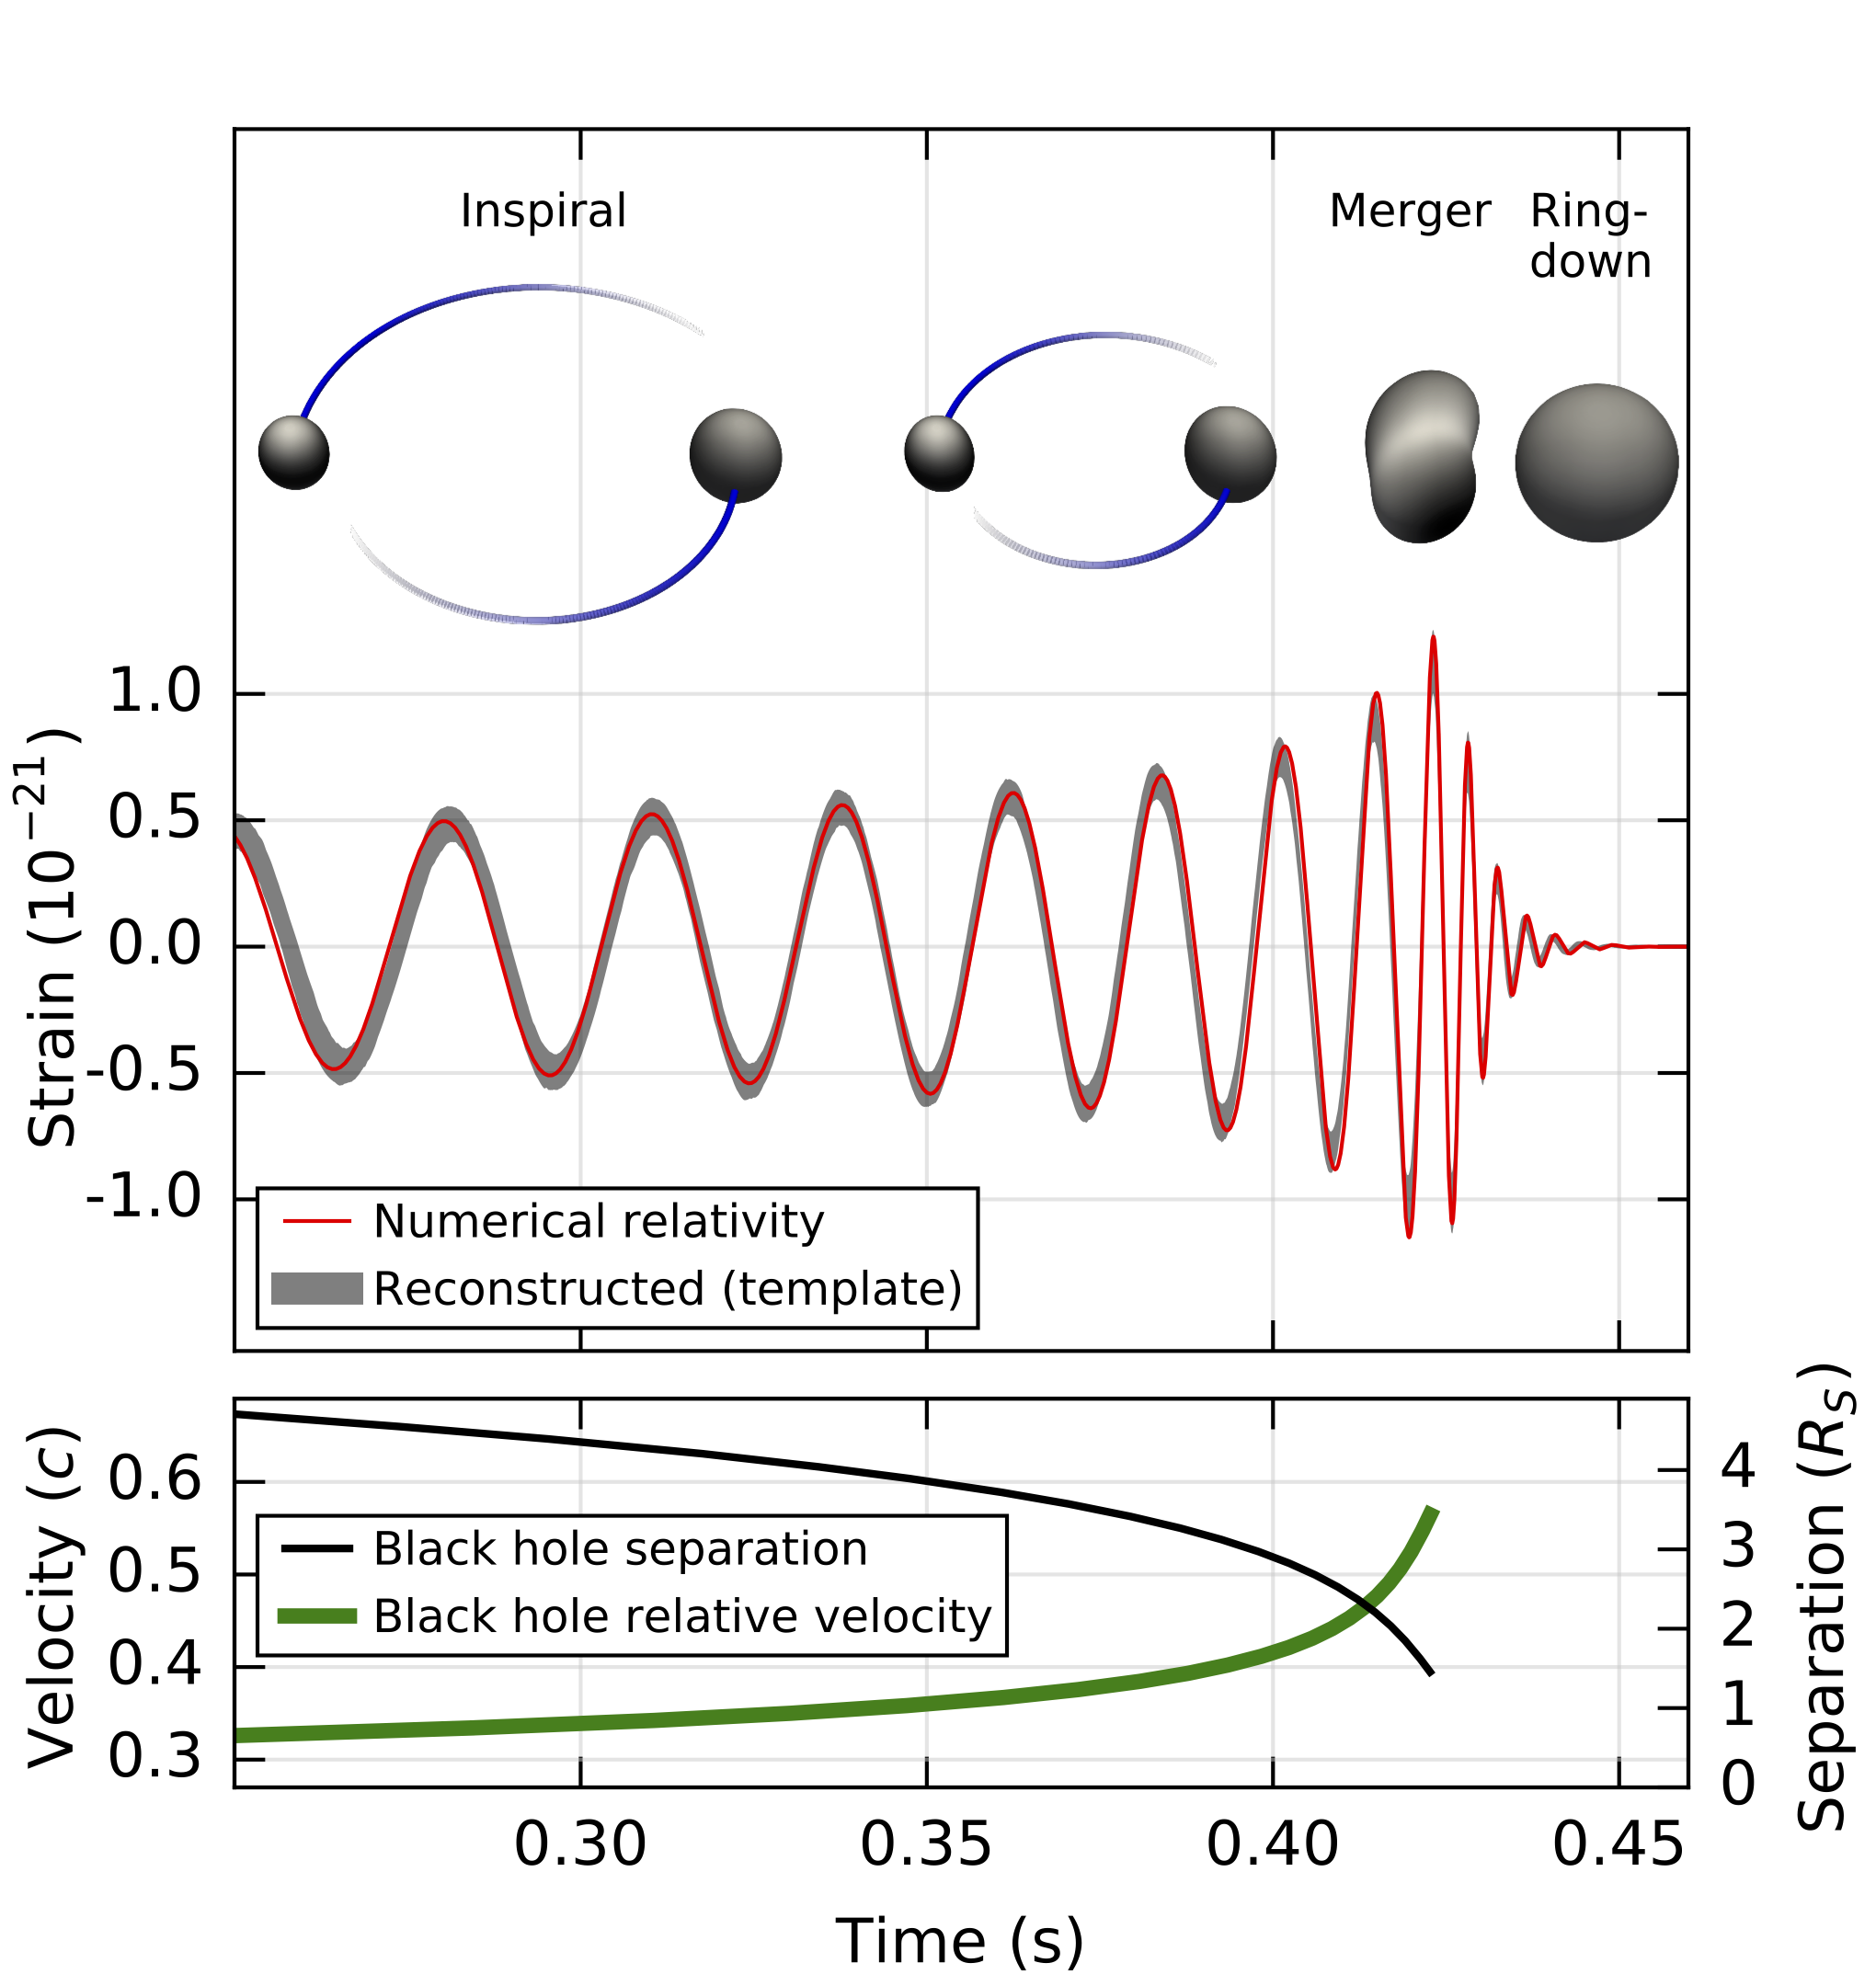
\includegraphics[width=0.5\linewidth]{sectionGW/inspiral.png}
  \caption{Figure issue de \cite{gw150914}. Panneau du haut: schéma de la phase d'inspiral, de fusion et de ringdown pour une binaire de trous noirs, ainsi que la forme des ondes émises au fil du processus. Panneau du bas: évolution de la séparation entre les trous noirs et de leur vitesse relative au cours du temps.}
  \label{fig:inspiral}
\end{figure}
%


\subsubsection*{Recherche d'évènements subissant un effet de lentille gravitationnelle}
Une lentille ravitationnelle est créée par un objet massif qui distord l'espace-temps.
L'effet des lentilles gravitationnelles est observé sur des ondes électromagnétiques.
Ces dernières sont déviées et créent pour l'observateur de multiples images de la source qui peuvent être magnifiées ou distordues.
Les ondes gravitationnelles sont également sujettes aux effets des lentilles gravitationnelles si la source, par exemple une CBC, est située derrière un objet massif.
Pour des objets très massifs, tel qu'un amas de galaxies, on parle alors de ``lentille massive'' ou encore ``lentille gravitationnelle forte''.
Pour des objets de masses plus faible, comme une étoile ou un objet compact, on parle de ``microlentille''.
On s'attend à ce que des lentilles fortes produisent de multiples signaux dans nos détecteurs que l'on verrait comme une forme d'onde qui se répète dans les données espacés de temps pouvant atteindre quelques mois.
Les lentilles forte ne devrait pas modifier l'évolution en fréquence des ondes gravitationnelles \cite{LVK_lensing}.
Grâce aux  multiples images les évènements subissant un effet de lentille gravitationnelle devrait permettre une meilleur localisation de leur source que les CBC habituels.
Les microlentilles pourraient quant à elles introduire un rythme de battement dans la forme d'onde \cite{lensing_beating}.
Cet effet pourrait apparaître si les conditions suivantes sont satisfaites:
\begin{itemize}
\item le delai temporel entre les différents chemin (qui produisent différentes images) doivent être du même ordre de grandeur que la période de l'onde gravitationnelle.
\item l'évènement doit être situé proche d'une caustique (ligne qui sépare les régions de différentes multiplicité d'images) afin d'être suffisamment magnifié pour permettre sa détection.
\end{itemize}

\subsubsection*{Recherche d'ondes continues}
Les ondes continues sont des ondes gravitationnelles observables sur une échelle de temps bien plus grande que celles provenant des CBC.
De possibles source d'ondes continues sont les étoiles à neutron en rotation avec une asymétrie ou une non-uniformité.
Les ondes continues émises par un tel système auraient une fréquence proche de la fréquence de rotation de l'étoile (ou du moins reliée à celle-ci).
Elles seraient donc quasiment monochromatiques avec des variation dûes à l'effet Doppler lié aux changements de la position de la source dans le ciel au cours du temps, ainsi qu'une évolution suivant le ``spin-down'' (ralentissement de la rotation) de l'étoile \cite{LVK_cw}.

Les recherches d'ondes continues peuvent être
\begin{itemize}
\item ciblées, c'est à dire que les données analysée proviennent d'une région du ciel où la présence d'une étoile à neutron en rotation est connue via l'observation d'un pulsar,
\item dirigées, en analysant des données provenant d'une régions spécifique du ciel dans laquelle il n'y a pas de source connue telle que le centre galactique,
\item globale ou ``all-sky'', visant à chercher des sources dans toutes les directions.
\end{itemize}

\subsubsection*{Recherches de bursts d'ondes gravitationnelles}
Les bursts sont des transient très courts qui peuvent durer de quelques secondes à quelques millisecondes.
Des source potentiels de burst d'ondes gravitationnelles sont les supernovae à effondrement de coeur, les excitations d'étoiles à neutrons, les cordes cosmiques \cite{LVK_burst}...
Les recherches de bursts peuvent utiliser des modèles de formes d'ondes comme les recherches CBC ou bien être des recherche sans modèle pour identifier les excès de puissance corrélés dans les détecteurs.

\subsubsection*{Recherche d'un bruit de fond stochastique d'ondes gravitationnelles}
Toutes les sources d'ondes gravitationnelles que nous ne détectons pas directement produisent tout de même des ondes qui peuvent nous atteindre.
Ces sources non résolues sont distribuées dans tout le ciel.
Les ondes qu'elles émettent devraient alors se superposer et créer un bruit de fond stochastique d'ondes gravitationnelles \cite{stochastic}.
Ce bruit de fond devrait être isotrope au premier ordre mais pourrait avoir de faibles fluctuations le rendant anisotrope comme le fond diffus cosmologique \cite{cmb}.
Des recherches pour un bruit de fond isotrope et anisotrope existent \cite{LVK_stochastic_aniso,LVK_stochastic_iso}.

%%%%%%%%%%
\subsection{Propriétés des ondes gravitationnelles et des CBC}

La forme d'onde des ondes gravitationnelles produites par une CBC est déterminée par les propriétés de la source, en particulier les masses et spins des deux objets de la binaire.
On appelle par convention masse1, spin1 et on écrit $m_1$, $s_1$ la masse et le spin de l'objet le plus lourd.
De même on appelle masse2, spin2 ($m_2$, $s_2$) la masse et le spin de l'objet le plus léger.
Dans les faits, on ne considère en général que la composante de spin orthogonale au plan de rotation de la binaire $s_{1,2z}$, et on note alors $s_{1,2}=s_{1,2z}$.
Les spins sont définis à partir du moment angulaire $J_{1,2}$ des deux objets et sont normalisés par les masses:
\begin{equation}
  s_i = \frac{J_i}{m^2_i} \text{  }, \text{  } i \in \{1,2\}
  \label{eq:spin}
\end{equation}
Ils prennent des valeurs entre $-1$ et $1$.

Nous définissons cinq quantités supplémentaire qui sont courament utilisées.
La masse totale
%
\begin{equation}
  M_{\textrm{tot}} = m_1 + m_2
\end{equation}
%
la masse réduite
%
\begin{equation}
  \mu = \frac{m_1 m_2}{M_{\textrm{tot}}}
\end{equation}
%
la masse chirp
%
\begin{equation}
  \mathcal{M} = m_{chirp} = \frac{ \left( m_1m_2 \right)^{\frac{3}{5}} }{ \left( m_1 + m_2 \right)^{\frac{1}{5}} } = \mu^{3/5}M_{\textrm{tot}}^{2/5}
  \label{eq:mchirp}
\end{equation}
%
le rapport des masses
%
\begin{equation}
  q=\frac{m_1}{m_2}
\end{equation}
%
et le spin effectif
%
\begin{equation}
  \chi_{\textrm{eff}} = \frac{s_1m_1\cos t_1 + s_2m_2\cos t_2}{m_1 + m_2} \stackrel{\textrm{\tiny (anti)aligned spins}}{=} \frac{s_1 m_1 + s_2 m _2}{m_1 + m_2}
  \label{eq:spin_eff}
\end{equation}
%
avec $t_1$ et $t_2$ les angles d'inclinaisons de chaque objet par rapport au moment orbital angulaire du système binaire.

%
Les ondes gravitationnelles peuvent être écrite comme le mélange de deux polarisations formant un angle de \SI{45}{\degree} \cite{polarization} appelées ``polarisation plus'', $h_+$, et ``polarisation croix'', $h_\times$, se rapportant aux directions dans lesquelles elles étendent et compressent l'espace.
La figure \ref{fig:polarization} montre leurs effets sur des particules ponctuelles.

Ces polarizations peuvent être écrites, pour un système CBC en orbite circulaire, comme \cite{Will_2014}
%
\begin{equation}
  \begin{split}
    h_+ =& -\frac{2\mathcal{M}}{R} (2\pi \mathcal{M} f_b)^{2/3} (1+\cos^2 i) \cos(2\Phi_b (t))\\
    h_\times =& -\frac{2\mathcal{M}}{R} (2\pi \mathcal{M} f_b)^{2/3} (2\cos i) \sin(2\Phi_b (t))
  \end{split}
  \label{eq:polarization}
\end{equation}
%
Où $i$ est l'inclinaison du système par rapport au plan du ciel, $f_b$ est la fréquence orbitale de la binaire et $\Phi_b(t) = 2\pi \int^t f_b(t') dt'$ est la phase orbitale.
$R$ est l'échelle charactéristique de distance au système.
Elle peut être prise comme la distance de luminosité
\begin{equation}
  D_L(z) = (1+z) \int_0^z \frac{dz'}{H(z')}
  \label{eq:luminosity_distance}
\end{equation}
où $z$ est le redshift, H le facteur de Hubble tel que $H = a^{-2} da/d\eta$ with $a(\eta)/a(\eta_0) = (1+z)^{-1}$ et $\eta$ est le temps conforme \cite{luminosity_distance}.
Ou encore la distance effective \cite{findchirp}
\begin{equation}
  D_{\textrm{eff}} = D \left( F_+^2 \left(\frac{1+\cos^2i}{2}\right)^2 +F_\times^2 \cos^2i \right)
  \label{eq:effective_distance}
\end{equation}
avec $F_+$ et $F_\times$ les réponses d'antennes de l'interféromètre aux polarisations plus et croix.
Les réponses d'antennes sont rapidement décrites dans le chapitre \ref{section:detection}.

Ce que l'on mesure sur Terre sont en fait les quantités redshiftées telles que la masse chirp redshiftée $\mathcal{M}_z = (1+z) \mathcal{M}$ et la fréquence redshiftée $f_z = f/(1+z)$.

% 
\begin{figure}
  \centering
  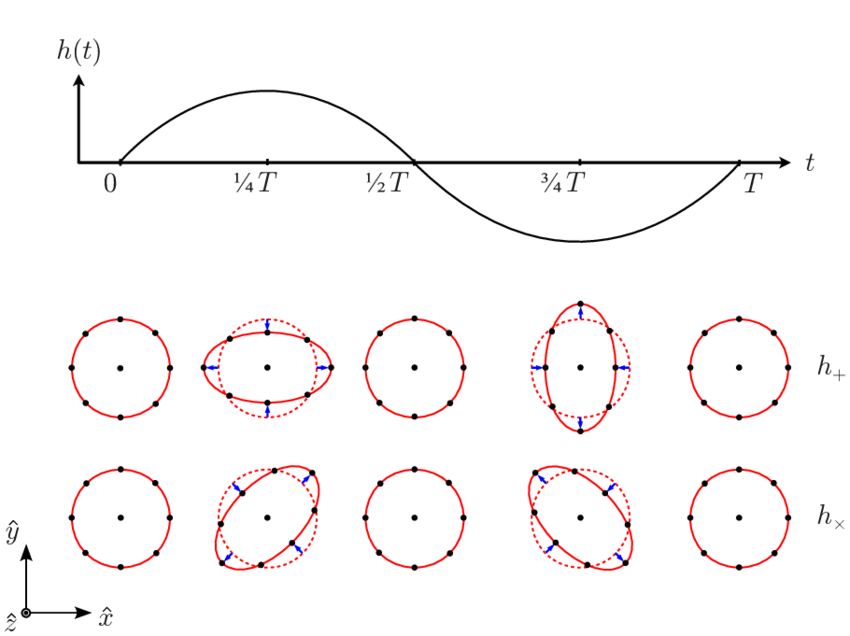
\includegraphics[width=0.5\linewidth]{sectionGW/polarization.png}
  \caption{Figure issue de \cite{polarization_novak}. Polarisations plus et croix d'une onde gravitationnelle se propageant selon l'axe z et leur effet sur un ensemble de particules ponctuelles en chute libre.}
  \label{fig:polarization}
\end{figure}
%


On voit en figure \ref{fig:waveform_mass} que plus le système binaire est lourd, plus le signal émis dans une certaine bande de fréquence est court.
On remarque également en figure \ref{fig:waveform_spin} que des spins élevé sont associés à des formes d'ondes plus longues, et que des spins anti-alignés sont associés à des formes d'ondes plus courtes.
Enfin, la figure \ref{fig:waveform_startFreq} montre l'impact du choix de la fréquence de début de génération de la forme d'onde sur la durée de celle-ci.
%
\begin{figure}
  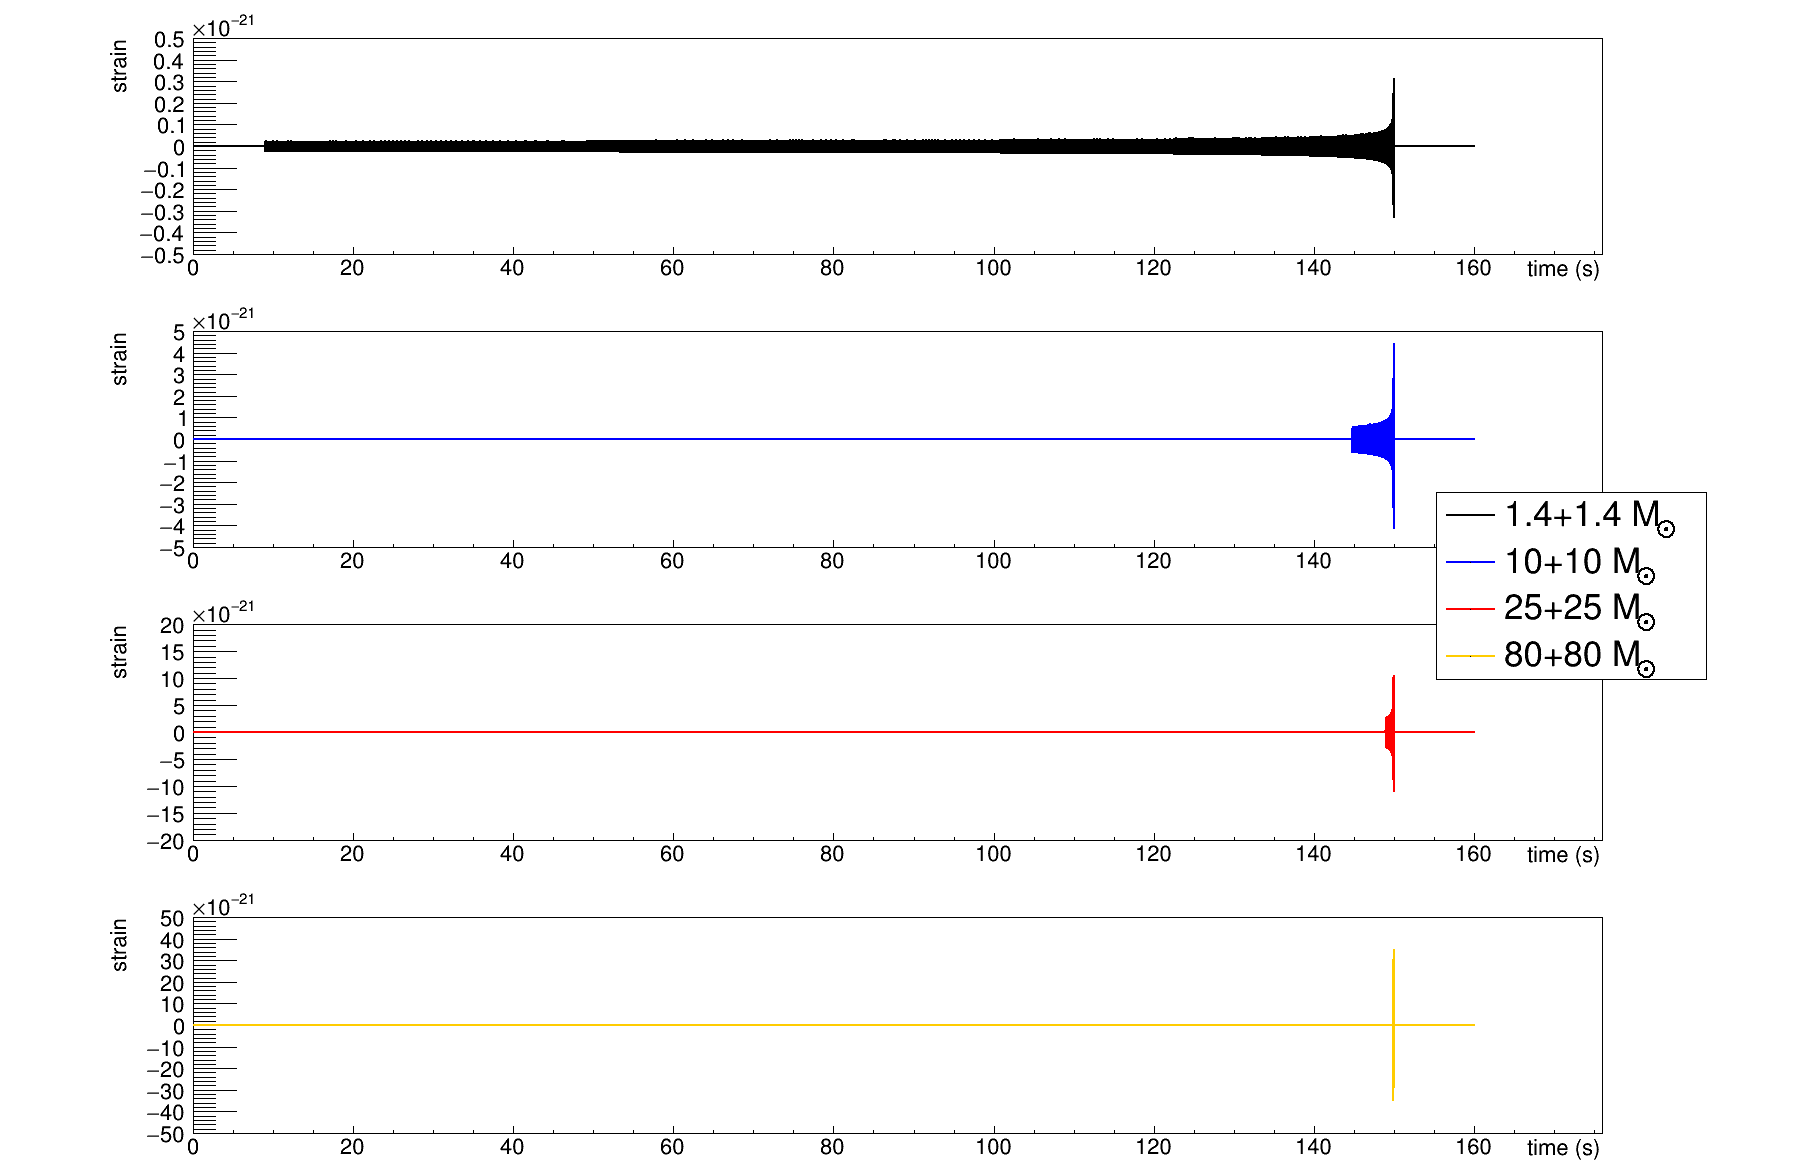
\includegraphics[width=\linewidth]{sectionGW/cWaveformMass.png}
  \caption{Forme d'onde pour des systèmes de différentes masses. Les autres paramètres sont spin1=spin2=0, fréquence de début de génération=\SI{21}{Hz}, distance effective=\SI{40}{Mpc}.}
  \label{fig:waveform_mass}
\end{figure}
% 
\begin{figure}
  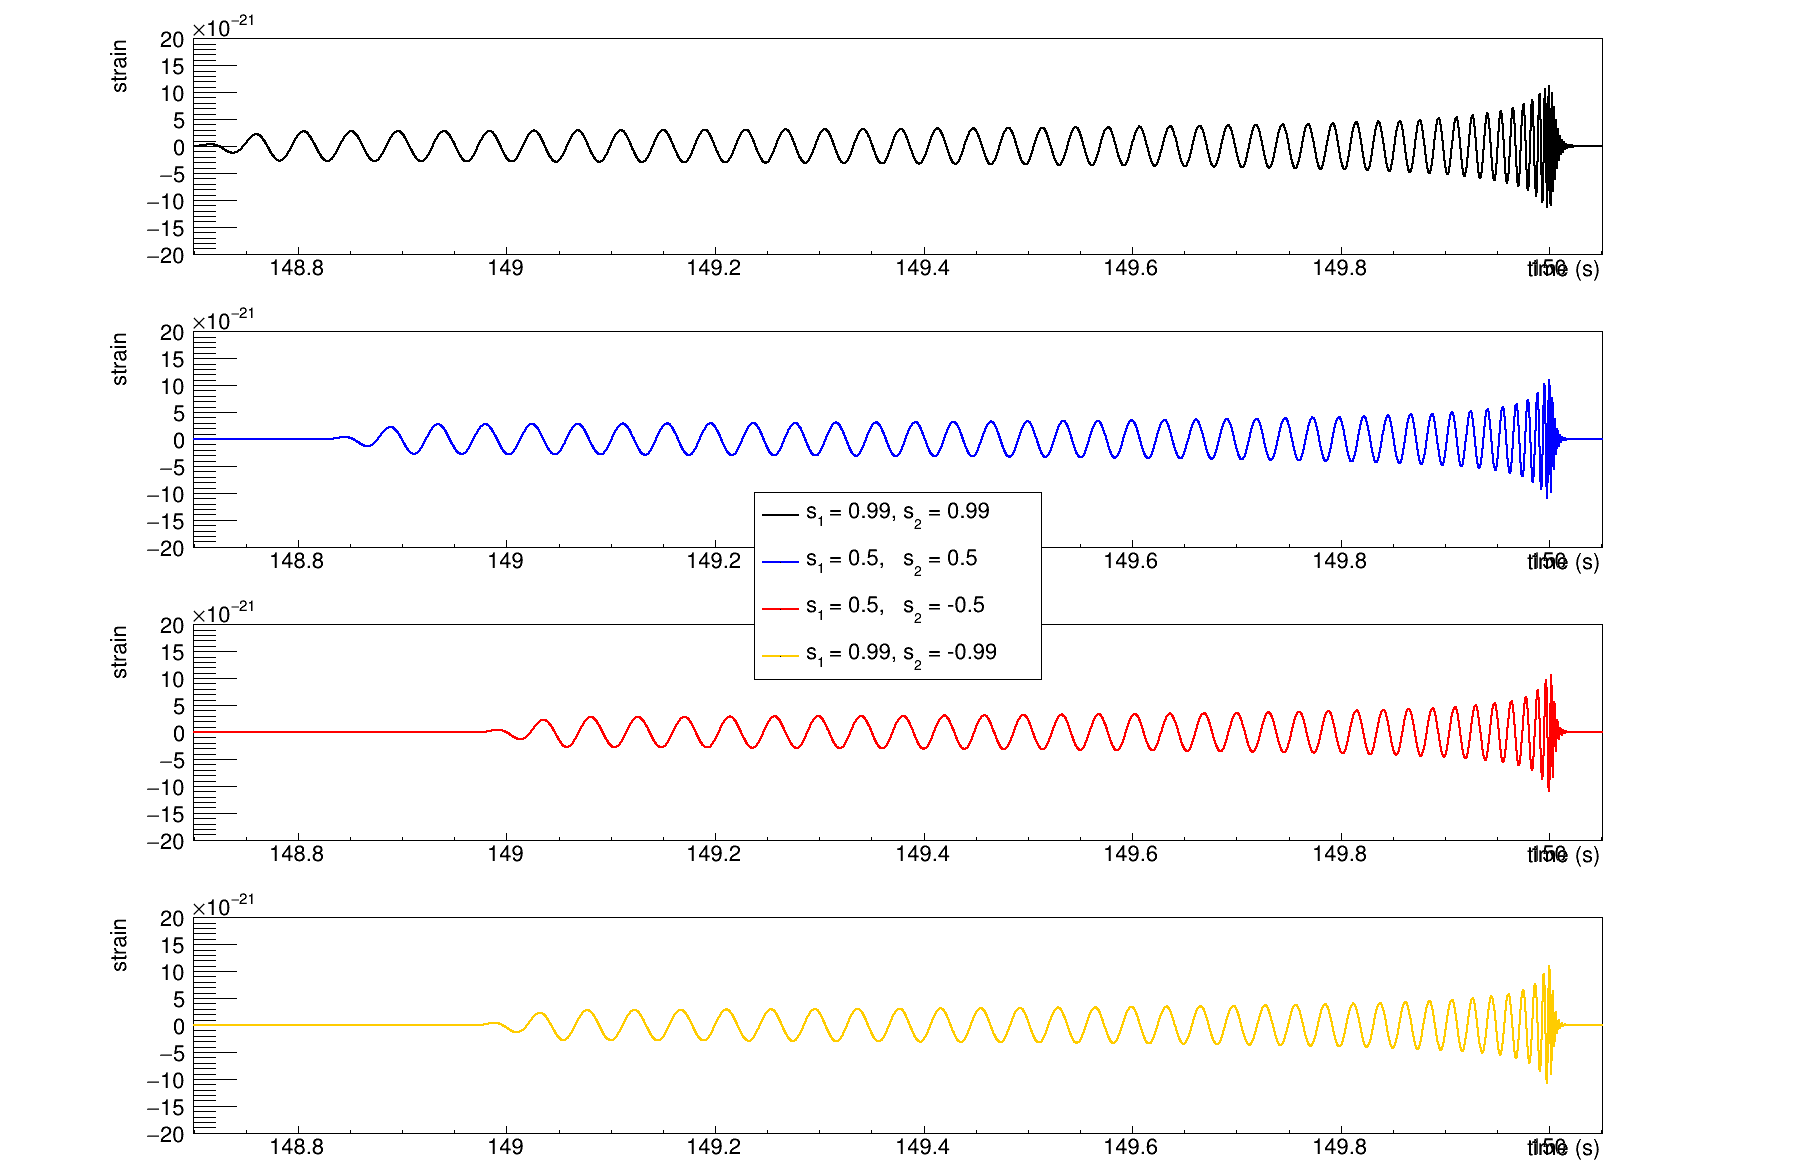
\includegraphics[width=\linewidth]{sectionGW/cWaveformSpin.png}
  \caption{Forme d'onde pour des systèmes avec différents spins. Les autres paramètres sont mass1=mass2=\SI{25}{\msun}, fréquence de début de génération=\SI{21}{Hz}, distance effective=\SI{40}{Mpc}.}
  \label{fig:waveform_spin}
\end{figure}
% 
\begin{figure}
  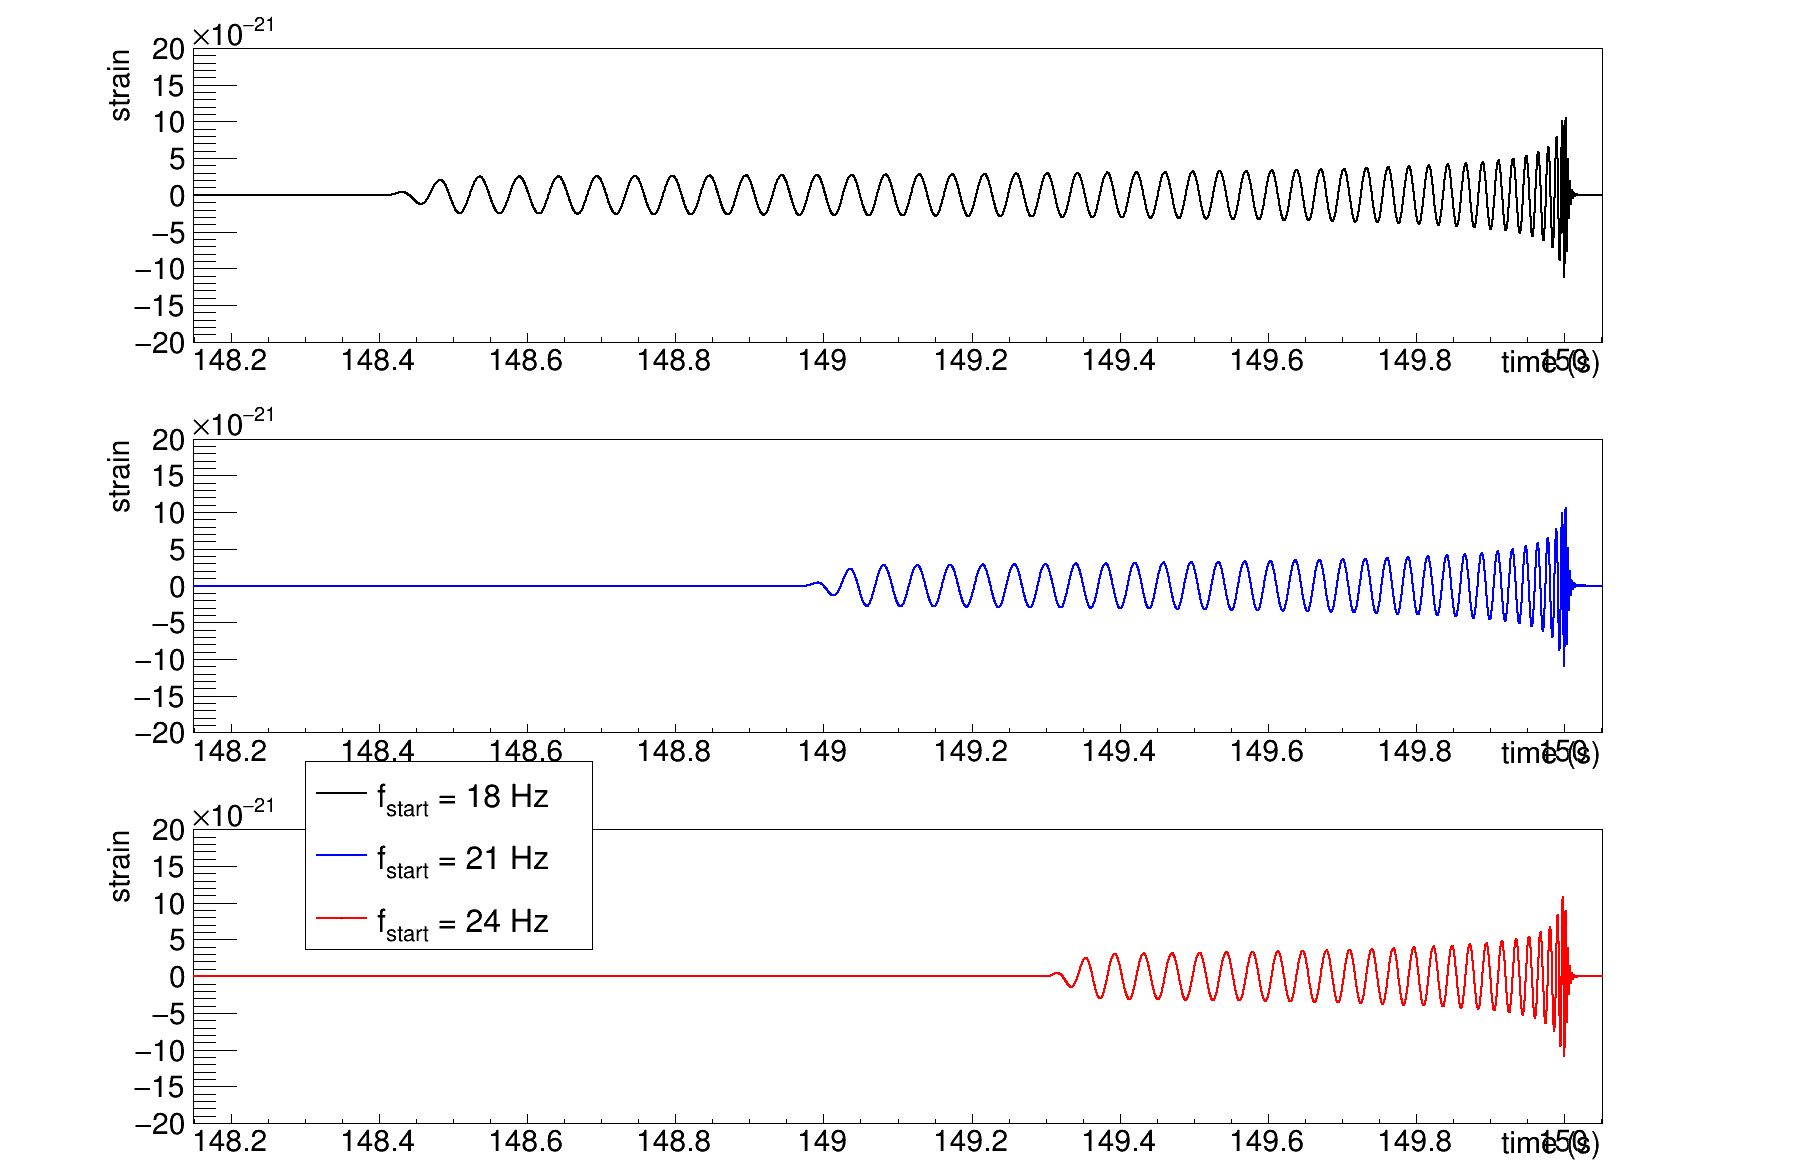
\includegraphics[width=\linewidth]{sectionGW/cWaveformFreq.png}
  \caption{Plot plusieurs waveform pour différentes valeurs de fréquence de début de génération pour un système de mass1=mass2=\SI{25}{\msun}, s1=s2=0 et distance effective=\SI{40}{Mpc}.}
  \label{fig:waveform_startFreq}
\end{figure}



%%%%%%%%%%
\subsection{Motivations pour la détection}
\label{sec:motivations}
En plus de la volonté de découvrir de nouveaux type de sources d'ondes gravitationnelles, de nombreuses motivations pour leur détection existent.
Nous en présentons ici les principales.

\subsubsection*{Astronomie multi-messager}
\label{sec:multimessenger}
Le but de l'astronomie multi-messager est de mieux comprendre les populations d'objets astrophysiques, leur évolution et leur environnement.
Le développement de l'astronomie multi-longueurs d'ondes a été motivé par le fait que différentes fréquences lumineuses fournissent différentes informations.
De la même manière, l'ajout des informations obtenues par l'observation (ou l'absence d'observation) de rayons cosmiques, neutrinos de haute énergie ou d'ondes gravitationnelles a enormément de valeur.
Un aperçu des jalons et découvertes multi-messagers est donné dans \cite{multimessenger}.
De nombreux efforts sont fournis pour faire des détections jointes de différent types de messagers.
Une association entre onde électromagnétique et neutrinos de haute énergie a été rapportée par plusieurs observatoire suite à la détection de neutrinos dont la position de la source était compatible avec un blazar de rayons $\gamma$ connu \cite{blazar_neutrino}.
La collaboration IceCube a également rapporté une preuve d'un excès de neutrinos compatibles avec la position d'une galaxie active proche \cite{agn_neutrino}.
Aucune détection jointe d'ondes gravitationnelles et neutrinos n'a été faite à ce jour \cite{hen_gw_antares,hen_gw_icecube}.
En revanche, une observation jointe d'ondes gravitationnelles et électromagnétiques s'est produite avec l'évènement GW170817 \cite{gw170817_multi,gw170817_multi_2}, la toute première détection d'une BNS qui fut alors suivie d'un sursaut gamma.
La détection d'onde gravitationnelle localisait la source dans une zone d'environ 31 degrés$^2$, à une distance de \SI{40}{Mpc} (suivie par d'autres mesures de la position de la source).
Le sursaut gamma a été détecté par plusieurs observatoires environ \SI{1.7}{s} après la fusion avec une localisation de la source dans une zone de 1100 degrés$^2$.
Des émissions d'ondes radios et de rayons X furent églament observées plusieurs jours après l'évènement.


\subsubsection*{Tests de la relativité générale}
\label{sec:testingGR}
% The list of tests given in this section is non-exhaustive and the reader is encouraged to read through the cited publications for more details.
La liste de tests donnée ici n'est pas exhaustive et plus de détails peuvent être trouvés dans les différentes oeuvres citées.

\vspace{0.2cm}
\textbf{Vitesse de propagation:} La relativité générale prédit que les ondes gravitationnelles se propagent non dispersivement à la vitesse de la lumière dans le vide.
Toute déviation serait donc un argument fort en faveur de théories alternatives de la gravité qui prédisent certaines variations de cette vitesse de propagation.
Elles pourraient être causées, par exemple, par le couplage des ondes avec des champs gravitationnels résiduels ou bien si la gravitation est associée à un champ massifs impliquant l'existence d'un graviton massif \cite{Will_1998,Will_2014,testingGR}.
D'un point de vu observationnel, une approche directe pour tester la vitesse de propagation des ondes gravitationnelles est de comparer leurs temps d'arrivée à ceux d'ondes électromagnétiques pour un même évènement.
Cela requiert toutefois une connaissance précise des temps d'émissions des deux.
La détection de GW170817 et du sursaut gamma associé GRB170817a a permis de contraindre la différence entre les vitesse de propagations ($\Delta v$) des ondes gravitationelles et de la lumière dans le vide ($c$) \cite{gw170817_multi_2}: $$-3 \times 10^{-15} \leq \frac{\Delta v}{c} \leq +7 \times 10^{-16}$$
Ce resultat a éliminé un certain nombre de théories alternatives de la gravitation.

\vspace{0.2cm}
\textbf{Polarisations:} Un autre test de la relativité générale consiste à chercher de nouvelles polarisations pour les ondes gravitationnelles.
En effet, la relativité générale ne permet que deux polarisation tensorielles tandis que d'autres théories en prédisent quatres additionnelles.
Il s'agirait de deux polarisations scalaires et de deux polarisations vectorielles \ref{fig:other_polarization}.
Ces autres polarisations sont recherchée en même temps que les ondes gravitationnelles continues \cite{other_polarization_cw}, le bruit de fond stochastique \cite{polarization} ainsi que des évènements CBC.
Des perspectives de recherches à l'aide de futurs détecteurs existent également \cite{testingGR,other_polarization_cbc}.

\vspace{0.2cm}
%\textbf{Deviation from waveforms predictions:} Waveforms are predicted by general relativity and used to look for signal in the detector output.
%Deviations are being searched for by looking at the residual power when substracting the predicted waveform of a detected signal to the data.
%A remaining excess of power would be an indicator of such deviation \cite{testingGR}.
\textbf{Déviations des prédictions de formes d'ondes:} Les formes d'onde sont prédites par la relativité générale et sont utilisées pour chercher du signal dans les données des détecteurs (see section \ref{sec:matched_filter}).
Des déviations sont recherchées en regardant la puissance résiduelle dans le détecteur après avoir soustrait au données la forme d'onde prédite d'un signal détecté.
Un excès de puissance suffisament significatif serait un indicateur de déviations.
%
\begin{figure}
  \centering
  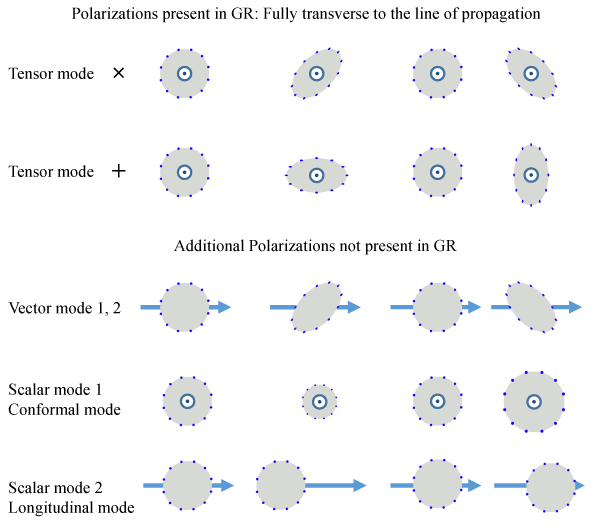
\includegraphics[width=0.6\linewidth]{sectionGW/other_polarization.png}
  \caption{Figure issue de \cite{other_polarization}. Polarisations ``$+$'' et ``$\times$'' ainsi que les autres types de polarisations qui ne sont pas prédits par la relativité générale.}
  \label{fig:other_polarization}
\end{figure}
%


\subsubsection*{Mesure de la constnte de Hubble}
\label{sec:H0}
La valeur de la constante de la constante de Hubble est une sujet très actif depuis de nombreuses années à causes des différences entre mesures directes et indirectes (correspondant à des distances différentes) qui sont en désaccords allant parfois jusqu'au niveau de $4-6\sigma$ level \cite{H0_1} comme montré en figure \ref{fig:H0}.

La constante de Hubble, $H_0$, est mesurée en étudiant la relation en distance et redshift pour des populations d'objets astrophysiques.
Des objets permettant une telle mesure sont appelés chandelles standards.
Il est possible de mesurer la distance de luminosité (eq. \ref{eq:luminosity_distance}) des sources CBC avec les ondes gravitationnelles mais il manque une mesure indépendante du redshift pour établir la relation de l'un en fonction de l'autre.
GW170817 était une chandelle standard grâce à la contrepartie électromagnétiques.
Cet évènement a permis de mesurer $H_0 = 70.0^{+12.0}_{-8.0}$ \si{km.s^{-1}.Mpc^{-1}} \cite{H0_gw170817}.
Pour les autres évènements on peut utiliser des catalogues de galaxies afin d'identifier la galaxie hôte ou, de manière plus réaliste, marginaliser sur de multiples potentielles galaxies hôtes pour obtenir une mesure indépendante du redshift.
Une analyse raffinée utilisant cette méthode a donné pour résultat $H_0 = 68.7^{+17.0}_{-8.3}$ \SI{}{km.s^{-1}.Mpc^{-1}} \cite{H0_LVK}.
Une mesure utilisant uniquement l'information onde gravitationnelle et se reposant sur les particularités des distributions de masse des CBC est également possible.
De futures mesures avec une meilleure précision va permettre de contraindre encore plus la valeurs de la constante de Hubble pour les modèles cosmologiques.
%
\begin{figure}
  \centering
  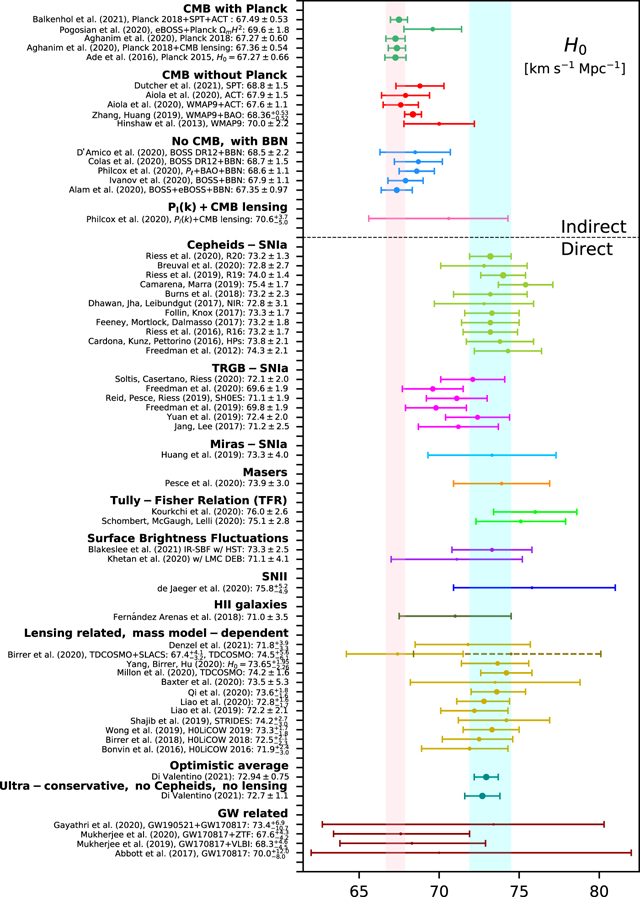
\includegraphics[width=0.7\linewidth]{sectionGW/measurementH0.jpg}
  \caption{Figure issue de \cite{H0_1}. Mesures directes et indirectes de $H_0$ avec intervalles à 68\% de niveau de confiance effectuées par diverses missions et collaborations. Traduit de \cite{H0_1}: ``La bande verticale cyan correspond à la valeur de H0 donnée par SH0ES \cite{shoes} (R20, $H0 = 73.2 \pm$ \SI{1.3}{km.s^{-1}.Mpc^{-1}} at 68\% CL) et la bande verticale rose correspond à la valeur de H0 rapportée par Planck 2018 \cite{Planck_2018} dans un scénario $\Lambda$CDM.''}
  \label{fig:H0}
\end{figure}
%

\subsubsection*{Contraintes sur l'équation d'état des étoiles à neutrons}
\label{sec:EOS}
L'équation d'état (EOS) des étoiles à neutrons relie les variables d'état telles que pression et densité entre elles et décrit la matière nucléaire à extrêmement haute densité à l'intérieur de l'étoile.
Elle est utilisée pour dériver de nombreuses propriété de l'étoile à neutrons telles que son rayon, sa masse, son moment d'inertie, sa déformabilité...
L'EOS permet également, en se basant sur les masses et populations d'étoiles à neutrons, de contraindre les mécanismes de formation des étoiles à neutrons.
De nombreux efforts ont été faits afin de développer des EOS permettant de décrire la matière d'une étoile à neutron de la croûte jusqu'au coeur intérieur.
Mais l'EOS est encore très peu contrainte et différentes approches donnent des équations différentes \cite{EOS_Douchin_2001,EOS_Lattimer_2001}.
Les expériences sur Terre qui visent à étudier la matière nucléaire à très faible température et forte densité ne peuvent pas reproduire les conditions de l'intérieur d'une étoile à neutron.
Il est donc impératif d'avoir recours à des observations astrophysiques via (de manière non exhaustive) les pulsars radios, les binaires à rayons X et, plus intéressant pour ce document, via les ondes gravitationnelles émises par les fusions d'étoiles à neutrons \cite{EOS_gw170817,EOS_pulsar,EOS_Lattimer_2021}.
La déformabilité causée par la force de marée de chacune des étoiles de la binaire sur l'autre est la quantité qui est la mieux mesurée pour contraindre l'EOS.
Elle est utilisée pour calculer les rayons des deux étoiles de la binaire.
En combinant ces mesures à celle des masses de la binaire il est possible de placer des contraintes sur l'équation d'état.

\subsubsection*{Taux et populations de CBC}
\label{sec:rateNpop}
Il est possible de considérer les évènements CBC non pas comme des évènements individuels mais comme une population de sources pour étudier leurs propriétés.
Cette considération est d'autant plus intéressante avec le début de O4 en Mai 2023 durant lequel on s'attend à plus de détections.
Les quantités que l'ont peut dériver de ces études sont par exemple le taux de merger des différents type de CBC et leur distribution en masse.
En utilisant le catalog GWTC-3 \cite{gwtc3}, les taux de fusions ont été rapportés dans \cite{rate_and_pop} entre
\begin{itemize}
\item \SI{10}{Gpc^{-3}.yr^{-1}} et \SI{1700}{Gpc^{-3}.yr^{-1}} pour des évènements BNS,
\item \SI{17.9}{Gpc^{-3}.yr^{-1}} et \SI{44}{Gpc^{-3}.yr^{-1}} pour des évènements BBH à redshift $z \leq 0.2$,
\item \SI{7.8}{Gpc^{-3}.yr^{-1}} et \SI{140}{Gpc^{-3}.yr^{-1}} pour des évènements NSBH.
\end{itemize}
%
Les distributions de masses rapportées sont
\begin{itemize}
\item uniforme entre  $1.2^{+0.1}_{-0.2}$ \si{\msun} et $2.0^{+0.3}_{-0.3}$ \si{\msun} pour les étoiles à neutrons,
\item loi de puissance avec pics à $\mathcal{M}_{c} = 8.3^{+0.3}_{-0.5}$ \si{\msun} et $\mathcal{M}_{c} = 27.9^{+1.9}_{-1.8}$ \si{\msun} pour les BBH.
\end{itemize}

\subsubsection*{Recherche de masses subsolaires}
\label{sec:ssm}
La découverte d'une objet compacte avec une masse inférieure à \SI{1}{\msun} serait la preuve de nouveaux mécanismes de formations d'objets compacts.
En effet les modèles actuels d'évolution stellaire pour les étoiles massives ne permettent un effondrement qu'en étoile à neutrons ou trou noir plus lourd que \SI{1}{\msun} \cite{ssm_O3a,ssm_O3b}.
Ces objets de masse subsolaire pourrait être des trou noirs primordiaux \cite{primordial_bh} ou bien des trous noirs formés par éffondrement de matière noire \cite{dm1,dm2,dm3} et indiquerait l'existence d'une nouvelle physique.
Des recherches de masses subsolaires sont menées par certaines chaînes d'analyses CBC avec un espace des paramètres dédié.
MBTA (chapitre \ref{section:mbta}) est l'un d'entre eux.

\subsubsection*{Recherche d'objets compacts exotiques}
\label{sec:exotic}
De nombreux objets compacts exotiques ont été théorisés, mais leur existance n'est toujours pas prouvée.
La forme d'onde crée par la coalescence de certains de ces objets est attendue comme identique à celle d'un signal BBH jusqu'à la phase de merger ou post-merger.
D'autres objets exotiques pourraient radier des ondes gravitationnelles par eux-même ou encore avoir un effet sur les ondes gravitationnelles comme du lensing \cite{ECO1,ECO2}.

% Des exemples d'objets compacts exotiques sont:
% \begin{itemize}
% \item les gravastars, introduits comme une solution alternative aux trou noirs comme produit final de l'éffondrement gravitationnel en un objet ponctuel \cite{gravastar1,gravastar2}.
% \item les trous de vers théorisés comme des distortions de l'espace-temps qui connecteraient des parties distantes de l'univers à l'instar d'un raccourci \cite{wormhole2,wormhole1}.
% \item Les étoiles à bosons, construites de l'association d'un champ scalaire et d'un champ gravitationnel. Elles consisteraient en des bosons stables ou non, tenus ensemble par interaction gravitationnelle.
% \item On peut également citer les fuzzballs \cite{fuzzball}, firewalls \cite{firewall} et trous noirs sans horizon \cite{horizonless_bh}.
% \end{itemize}


